\section{Introduction}

% Reproducibility is more important than it is hard
The importance of reproducibility outweighs its difficulty. While wrestling
with large amounts of data, millions of lines of code, and diverse developer
groups, it is extremely  hard to remember to make workflows understandable, let
alone reproducible. But our research group has found  that the benefits of
reproducibility, from a research, educational, and productivity standpoint,
make the pain points worth it. After all, the scientific method requires such
practices  and other fields have been emphasizing the reproducibility of
experimental results for {\it centuries}; it is about time that the field of
computer systems change its {\it ad-hoc} workflows to be more reproducible.

% Not incentivized
Once we adopted this philosophy, the road to reproducible research and paper
artifacts was not smooth.  We use the Popper
convention~\cite{jimenez:ipdpsw17-popper} because of its focus on open-source
cluster management toolkits. Our workflow uses the DevOps tools shown in
Figure~\ref{fig:workflow} and is described in more detail in
Section~\S\ref{sec:popper-compliant-papers}. We have produced four
Popper-compliant papers, three of which have been published in the proceedings
of top conferences.

\begin{figure}[tb] 
  \centering
  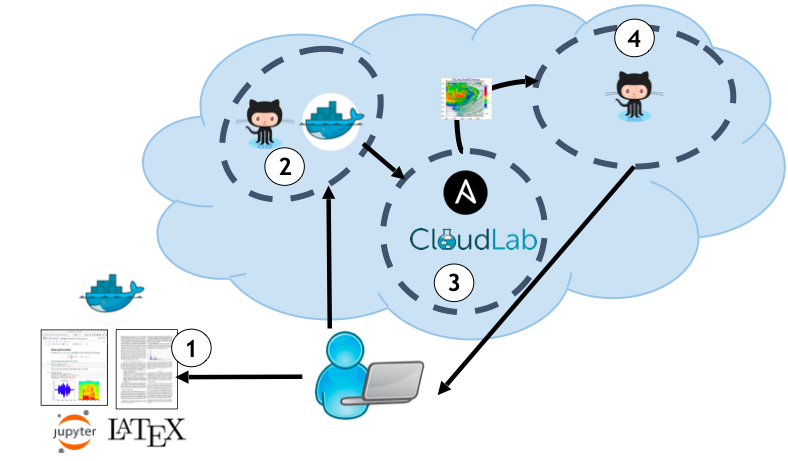
\includegraphics[width=1\linewidth]{./figures/workflow.png}
  \caption{Illustration of the workflow used in our papers; Figure is
adapted from~\cite{jimenez:ipdpsw17-popper}. For (1) - the visualization
component - we use Jupyter, \LaTeX, and Docker; for (2) - the code component -
we use GitHub and Docker; for (3) - the multi-node component - we use Ansible
and CloudLab; and for (4) - the data set component - we use GitHub.}
  \label{fig:workflow}
\end{figure}


\begin{table*}[t]
\centering
\normalsize
\begin{tabular}{ >{}m{3.2in} | c | >{}m{2.9in} }
&\\
\multicolumn{1}{c|}{Paper [Reference]} & Status & Reason\\ \hline
&\\
Malacology: A Programmable Storage System~\cite{sevilla:eurosys17-malacology}
& PASS
& Reproducing results on different clusters not tested\\ 
&\\\hdashline
&\\
Cudele: An API and Framework for Programmable Consistency and Durability in a Global Namespace~\cite{sevilla:ipdps18-cudele}
& GOLD 
& Tested on multiple clusters, READMEs for re-running experiments provided\\
&\\\hdashline
&\\
Programmable Caches with a Data Management Language \& Policy Engine~\cite{sevilla:ccgrid18-parsplice}
& FAIL 
& Security issues with public facing repositories and private networks/systems\\
&\\\hdashline
&\\
Tintenfisch: File System Namespace Schemas and Generators~\cite{sevilla:techreport18-tintenfisch}
& GOLD 
& No performance results, just software replicability needed\\
&\\
\end{tabular}

\caption{Papers following the Popper Convention. The statuses are
from~\cite{jimenez:rr18-popper}, where GOLD means results are reproducible,
PASS means experiments run, and FAIL means experiment artifacts are available
(but may not run). We graded the repositories based on our own internal
evaluations -- ideally, this evaluation would be done by someone outside the
team, like a paper reviewer or a member of the conference committee. Over time,
our Popper-compliance has improved, except for the work we did
in~\cite{sevilla:ccgrid18-parsplice}, which faced security obstacles (see
Section~\S\ref{sec:reqs}).}

\label{table:papers}
\end{table*}

% Contributions
While our experience with these state-of-the-art
DevOps tools have been delightfully straightforward, which is no doubt a
testament to the importance of reproducibility in real, large-scale clusters,
our struggle composing these tools together in a coherent way has been a real
challenge.  From designing workflows with these tools, we have developed a list
of pitfalls that wasted time and effort. Our contributions are as follows:

\begin{itemize}

  \item the structure and workflow of some of our papers,
using a baseline template designed for the Ceph~\cite{weil:osdi2006-ceph}
storage system (Section~\S\ref{sec:popper-compliant-papers}).

  \item three pitfalls for reproducibility that severely limited
productivity in early papers; designing best practices that address these
pitfalls before starting the project saved us time and effort in subsequent
research explorations (Section~\S\ref{popper-best-practices}).

  \item a call-to-arms for the downfall of practices that fly in the face of
reproducibility. We highlight difficulties with academic conferences, work at
national laboratories, and work in industry because that is where we have the
most experience (Section~\S\ref{sec:community-cooperation}).

\end{itemize}

We give each of our paper repositories a status using the convention
in~\cite{jimenez:rr18-popper}: GOLD means that results are fully reproducible,
PASS means the experiments will run, and FAIL means that experiments are not
guaranteed to execute. A FAIL status is still Popper-compliant because
experiment artifacts and results are available.  Over time, our Popper status
has improved from PASS to GOLD because we were able to shape our best practices
from our observed pitfalls. We also learned that going back and making
published papers Popper-compliant is too difficult and is not incentivized, as
described in Section~\S\ref{sec:repro}. The one FAIL status we have can be
attributed to security issues we had working at a national laboratory, as
described in more detail in Section~\S\ref{sec:reqs}. It is our hope that the
pitfalls we stumbled over can be used as a best practices guide for future
articles.

